\input{$UNI_DIR/msc/tex/HWSetup}
\input{$UNI_DIR/msc/tex/EngBindings}

%
% Homework Details
%   - Title
%   - Subtitle
%   - Due date
%   - Due time
%   - Course
%   - Section/Time
%   - Instructor
%   - Author
%

\newcommand{\hmwkTitle}{HW03}
\newcommand{\hmwkSubTitle}{System Propagation}
\newcommand{\hmwkDueDate}{October 30th. 2025}
\newcommand{\hmwkDueTime}{09:30 AM}
\newcommand{\hmwkClass}{ENAE 441 - 0101}
\newcommand{\hmwkClassTime}{09:30 AM}
\newcommand{\hmwkClassInstructor}{Dr. Martin}
\newcommand{\hmwkAuthorName}{\textbf{Vai Srivastava}}
\newcommand{\hmwkCompletionDate}{\today}

\begin{document}

\maketitle

\pagebreak

\begin{hwkProblem}{1}{Propagation Functions \textit{(30 pts.)}} \label{hwk:p01}

	Please implement the following functions in your code to confirm your understanding of the different propagation strategies. You are not required to use these exact functions in subsequent questions, as there may be more appropriate / efficient implementations for subsequent questions. They are merely provided as a way to confirm your own understanding of the process.
	\begin{enumerate}[label=(\alph*)]
		\item \label{hwk:p01a} Write a function that propagates a LTI system forward numerically\footnote{using Python's \mintinline{python}{scipy.integrate.solve_ivp}} and plot the displacement \(x(t)\) and velocity \(\dot{x}(t)\).
		\item \label{hwk:p01b} Write a function that propagates a LTI system forward analytically using a continuous time (CT) STM\footnote{Be sure to use \mintinline{python}{scipy.linalg.expm} to make the matrix exponential}.
		\item \label{hwk:p01c} Write a function that propagates a LTI system forward analytically using a discrete time (DT) STM\footnote{Be sure to use \mintinline{python}{numpy.linalg.matrix_power} to raise the matrix to a power}.
		\item \label{hwk:p01d} Write a function that propagates a LTV system by jointly integrates the nominal trajectory and the state transition matrix for a fixed amount of time\footnote{Hint: Form a joint state-STM vector \(\boldsymbol{z}={\begin{bmatrix}\fn*{\boldsymbol{x}_{\text{nom}}}[t] & \fn*{\phi}[t, t_0]\end{bmatrix}}^{\top}\). Unroll the STM into a single column vector such that the object passed to \mintinline{python}{solve_ivp} is a single column vector. Use \(\fn*{\bm{\Phi}}[t_0, t_0]=\mathcal{I}_{6\times6}\) for the initial condition}.
		\item \label{hwk:p01e} Write a function that returns the maximum allowable sampling time for a discrete time system to avoid aliasing.
	\end{enumerate}

	\hwkSol{} \label{hwk:s01}

	\hwkPart{} \label{hwk:s01a}

	\inputminted[firstline=122, lastline=153]{python}{./src/hw03.py}

	\hwkPart{} \label{hwk:s01b}

	\inputminted[firstline=156, lastline=169]{python}{./src/hw03.py}

	\hwkPart{} \label{hwk:s01c}

	\inputminted[firstline=172, lastline=191]{python}{./src/hw03.py}

	\hwkPart{} \label{hwk:s01d}

	\inputminted[firstline=194, lastline=221]{python}{./src/hw03.py}

	\hwkPart{} \label{hwk:s01e}

	\inputminted{python}{./outputs/text/s01e.txt}

	\hwkCode{} \label{code:s01}

	See the \href{https://www.github.com/vaisriv/enae441-hw03/blob/main/src/hw03.py#L118}{Python code} for this assignment.

\end{hwkProblem}

\begin{hwkProblem}{2}{Continuous Time Linear System \textit{(30 pts.)}} \label{hwk:p02}

	Consider a spring-mass-damper system
	\[
		m \fn*{\ddot{x}}[t] + c \fn*{\dot{x}}[t] + k \fn*{x}[t] = 0
	\]
	with system mass \(m = 1\), damping coefficient \(c = \qty{0.5}{\N\s\per\m}\), and spring constant \(k = \qty{4}{\N\per\m}\) and an initial condition of \(\fn*{\boldsymbol{x}}[0] = \cbvect{1}{0}\).

	The system is measured by observing the position
	\[
		\fn*{y}[t] = \fn*{x}[t]
	\]
	\begin{enumerate}[label=(\alph*)]
		\item \label{hwk:p02a} Express the system as a continuous-time state-space model and as a discrete-time model. Define a state vector of \(\fn*{\boldsymbol{x}}[t] = \cbvect{\fn*{x}[t]}{\fn*{\dot{x}}[t]}\) and define all of the corresponding matrices. Assume no external input (\(\fn*{\boldsymbol{u}}[t] = 0\)).
		\item \label{hwk:p02b} Propagate the system forward for 10 seconds using all three LTI propagation methods and plot \(\fn*{x}[t]\) and \(\fn*{\dot{x}}[t]\) on the same figure.
		\item \label{hwk:p02c} Compare the results. What happens when you apply a \(\Delta t\) value that exceeds the critical threshold in the DT STM?
		\item \label{hwk:p02d} Use the set of position measurements in \mintinline{bash}{HW3-spring-data.npy} to determine the initial state \(\fn*{\boldsymbol{X}}[t=0]\) for a different trajectory.
		\item \label{hwk:p02e} How many measurements are needed to ensure the state \(\fn*{\boldsymbol{x}}[t]\) is observable if \(\Delta t=\qty{1}{\s}\)? Explain your findings.
	\end{enumerate}

	\hwkSol{} \label{hwk:s02}

	\hwkPart{} \label{hwk:s02a}

	With state \(x(t)=\left[\begin{array}{l}x(t) \\ \dot{x}(t)\end{array}\right]\) and output \(y(t)=x(t)\), the continuous-time model is

	\[
		\dot{x}(t)=\mathbf{A} x(t), \quad \mathbf{A}=\left[\begin{array}{cc}
				0            & 1            \\
				-\frac{k}{m} & -\frac{c}{m}
			\end{array}\right]=\left[\begin{array}{cc}
				0  & 1    \\
				-4 & -0.5
			\end{array}\right], \quad \mathbf{C}=\left[\begin{array}{ll}
				1 & 0
			\end{array}\right], \quad \mathbf{D}=\mathbf{0}
	\]

	For a sampling period \(\Delta t\), the discrete-time model (no input) is

	\[
		x_{k+1}=\mathbf{A}_d x_k, \quad y_k=\mathbf{C} x_k,
	\]

	with \(\mathbf{A}_d=e^{\mathbf{A} \Delta t}=\Phi(\Delta t)\)

	Because this is a 2nd-order underdamped oscillator, it's convenient to write \(\alpha= \frac{c}{2 m}=\frac{1}{4}, \omega_n=\sqrt{k / m}=2\), and \(\omega_d=\omega_n \sqrt{1-\zeta^2}=2 \sqrt{1-\left(\frac{c}{2 m \omega_n}\right)^2}=\) 1.98431348.

	The continuous-time STM is

	\[
		\Phi(t)=e^{-\alpha t}\left[\begin{array}{cc}
				\cos{\omega_d t}+\frac{\alpha}{\omega_d} \sin{\omega_d t} & \frac{1}{\omega_d} \sin{\omega_d t}                       \\
				-\frac{\omega_n^2}{\omega_d} \sin{\omega_d t}             & \cos{\omega_d t}-\frac{\alpha}{\omega_d} \sin{\omega_d t}
			\end{array}\right]
	\]

	Hence the discrete state matrix is \(\mathbf{A}_d=\boldsymbol{\Phi}(\boldsymbol{\Delta} t)\) with the same \(\alpha, \omega_n, \omega_d\) substituted, and \(\mathbf{C}_d=\mathbf{C}, \mathbf{D}_d=\mathbf{D}=\mathbf{0}\)
	
	\pagebreak

	\hwkPart{} \label{hwk:s02b}

	\begin{figure}[H] \label{fig:s02b}
		\begin{center}
			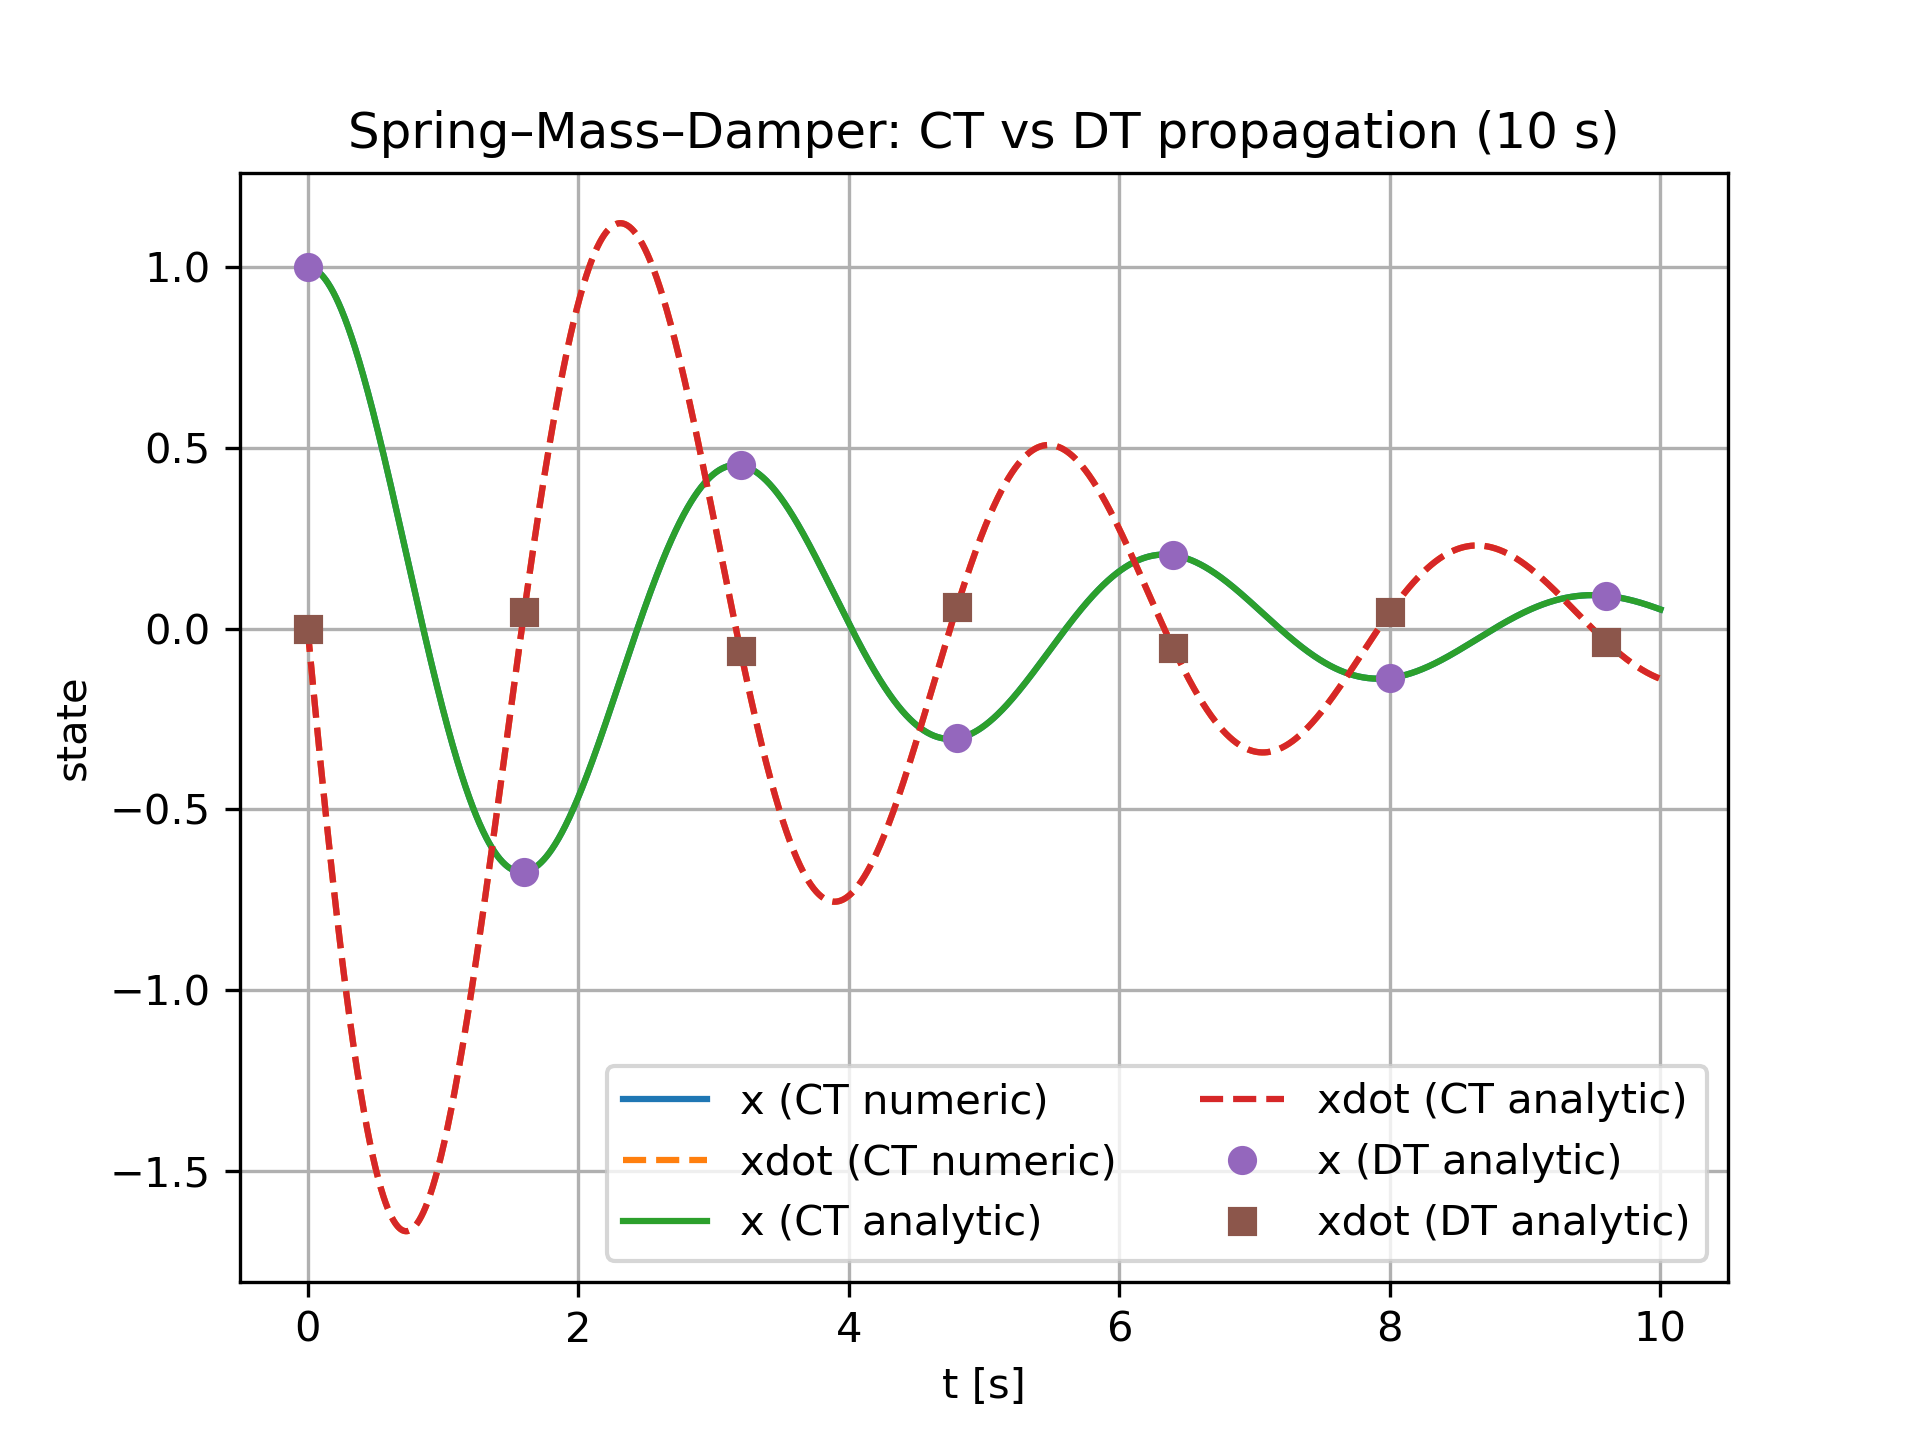
\includegraphics[width=0.45\textwidth]{./outputs/figures/s02b.png}
		\end{center}
		\caption{Propagation Trajectories}
	\end{figure}

	\hwkPart{} \label{hwk:s02c}

	\inputminted{python}{./outputs/text/s02c.txt}

	\hwkPart{} \label{hwk:s02d}

	\inputminted{python}{./outputs/text/s02d.txt}

	\hwkPart{} \label{hwk:s02e}

	\inputminted{python}{./outputs/text/s02e.txt}

	\hwkCode{} \label{code:s02}

	See the \href{https://www.github.com/vaisriv/enae441-hw03/blob/main/src/hw03.py#L234}{Python code} for this assignment.

\end{hwkProblem}

\begin{hwkProblem}{3}{Continuous Time Non-Linear System \textit{(40 pts.)}} \label{hwk:p03}
	Consider a satellite in a 3D Keplerian orbit around Earth. The dynamics of the satellite can be modeled using Newton's second law under the gravitational force:
	\[
		\ddot{\boldsymbol{r}}=-\frac{\mu}{r^3} \boldsymbol{r},
	\]
	where \(\mu=\qty{398600}{\km\cubed\per\s\squared}\) is the Earth's gravitational parameter and \(\boldsymbol{r}\) is the position vector of the satellite in the Earth-centered inertial (ECI) frame.

	The initial position and velocity vectors are:
	\[
		{}^{\mathcal{N}} \fn*{\boldsymbol{X}}[0]=\left[\begin{array}{c}
				\qty{7000}{\km}      \\
				\qty{0.0}{\km}       \\
				\qty{0.0}{\km}       \\
				\qty{0.0}{\km\per\s} \\
				\qty{7.5}{\km\per\s} \\
				\qty{3.5}{\km\per\s}
			\end{array}\right]^{\top}
	\]
	and the measurement function of the system is the range, \(\rho\) taken from an observer at \(\phi=\qty{30}{\deg}\) latitude and \(\lambda=\qty{60}{\deg}\) longitude, where the radius of the Earth, \(R_E\) is taken as \qty{6378}{\km} and the rotation of the Earth is \(\omega_{E / N}=\qty{7.2921150e-5}{\rad\per\s}\). Define the state vector as \(\fn*{\boldsymbol{x}}[t]={\rbvect{\fn*{\boldsymbol{r}}[t]}{\fn*{\boldsymbol{v}}[t]}}^{\top}\).

	\begin{enumerate}[label=(\alph*)]
		\item \label{hwk:p03a} Linearize the system around a nominal trajectory \( \fn*{X_{\text{nom}}}[t] \), deriving the system and output matricies \( A = \pdrv{\bm{f}}{\bm{x}} \) and \( C = \pdrv{\bm{h}}{\bm{x}} \).
		\item \label{hwk:p03b} Write a function that outputs \( A_{k} \).
		\item \label{hwk:p03c} Write a function that outputs \( C_{k} \).
		\item \label{hwk:p03d} Numerically propagate (i) the nominal trajectory and (ii) the nominal trajectory perturbed an initial state deviation of \( \delta \bm{X} = {\left[30, 0, 0, 0, 0, 0.1\right]}^{\top} \) for 90 minutes. Plot the difference in the position vector \( \fn*{\delta r}[t] \) as a function of time.
		\item \label{hwk:p03e} Propagate the state deviation directly using the integrated state transition matrix from the augmented nominal state vector (i.e. \hyperref{hwk:p01d}{Problem 1.D}) and plot the position vector deviation as a function of time.
		\item \label{hwk:p03f} Increase the initial state perturbation to \( \delta \bm{X} = {\left[1000, 0, 0, 0, 0, 0.1\right]}^{\top} \) and integrate (i) numerically and (ii) using the STM. Plot \( \fn*{\delta r}[t] \) for both propagatation strategies.
		\item \label{hwk:p03g} Explain what you see.
		\item \label{hwk:p03h} A set of range measurements are provided for a different trajectory in \mintinline{bash}{HW3-kepler-data.npy} from the same observer. Use the mesaurements to estimate the initial state deviation \( \fn*{\delta \bm{x}}[t_{0}] \) using the same nominal trajectory as before.
		\item \label{hwk:p03i} Explain your approach.
	\end{enumerate}

	\hwkSol{} \label{hwk:s03}

	\hwkPart{} \label{hwk:s03a}

	State: \(\boldsymbol{x}=[\boldsymbol{r} ; \boldsymbol{v}] \in \mathbb{R}^6\), dynamics

	\[
		\dot{x}=\left[\begin{array}{l}
				\dot{r} \\
				\dot{v}
				\end{array}\right]=\left[\begin{array}{c}
				v \\
				-\frac{\mu}{\|r\|^3} r
		\end{array}\right]=: f(x)
	\]

	Let \(r=\|\boldsymbol{r}\|\). The Jacobian is

	\[
		\mathbf{A}=\frac{\partial f}{\partial x}=\left[\begin{array}{cc}
				\mathbf{0}_{3 \times 3} & \mathbf{I}_{3 \times 3} \\
				\mu\left(\frac{3 r r^{\top}}{r^5}-\frac{\mathbf{I}_{3 \times 3}}{r^3}\right) & \mathbf{0}_{3 \times 3}
		\end{array}\right]
	\]

	Measurement: range to a ground observer \(\rho=\left\|\boldsymbol{r}-\boldsymbol{r}_{\text {obs }}(\boldsymbol{t})\right\|\)

	Hence

	\[
		\mathbf{C}=\frac{\partial \rho}{\partial x}=\left[\begin{array}{ll}
				\frac{\left(r-r_{\text{obs}}(t)\right)^{\top}}{\left\|r-r_{\text{obs}}(t)\right\|} & \mathbf{0}_{1 \times 3}
		\end{array}\right]
	\]

	The observer position in ECI (with latitude \(\phi\), longitude \(\lambda\), Earth radius \(R_E\), rotation rate \(\omega_E\) ) is

	\[
		r_{\text{obs}}^{\mathrm{ECI}}(t)=\mathbf{R}_3\left(\omega_E t\right)\left[\begin{array}{c}
				R_E \cos{\phi} \cos{\lambda}\\
				R_E \cos{\phi} \sin{\lambda}\\
				R_E \sin{\phi}
				\end{array}\right], \quad \mathbf{R}_3(\theta)=\left[\begin{array}{ccc}
				\cos{\theta} & -\sin{\theta} & 0 \\
				\sin{\theta} &  \cos{\theta} & 0 \\
				0 & 0 & 1
		\end{array}\right]
	\]

	\hwkPart{} \label{hwk:s03b}

	\inputminted{python}{./outputs/text/s03b.txt}

	\hwkPart{} \label{hwk:s03c}

	\inputminted{python}{./outputs/text/s03c.txt}

	\pagebreak

	\hwkPart{} \label{hwk:s03d}

	\begin{figure}[H] \label{fig:s03d}
		\begin{center}
			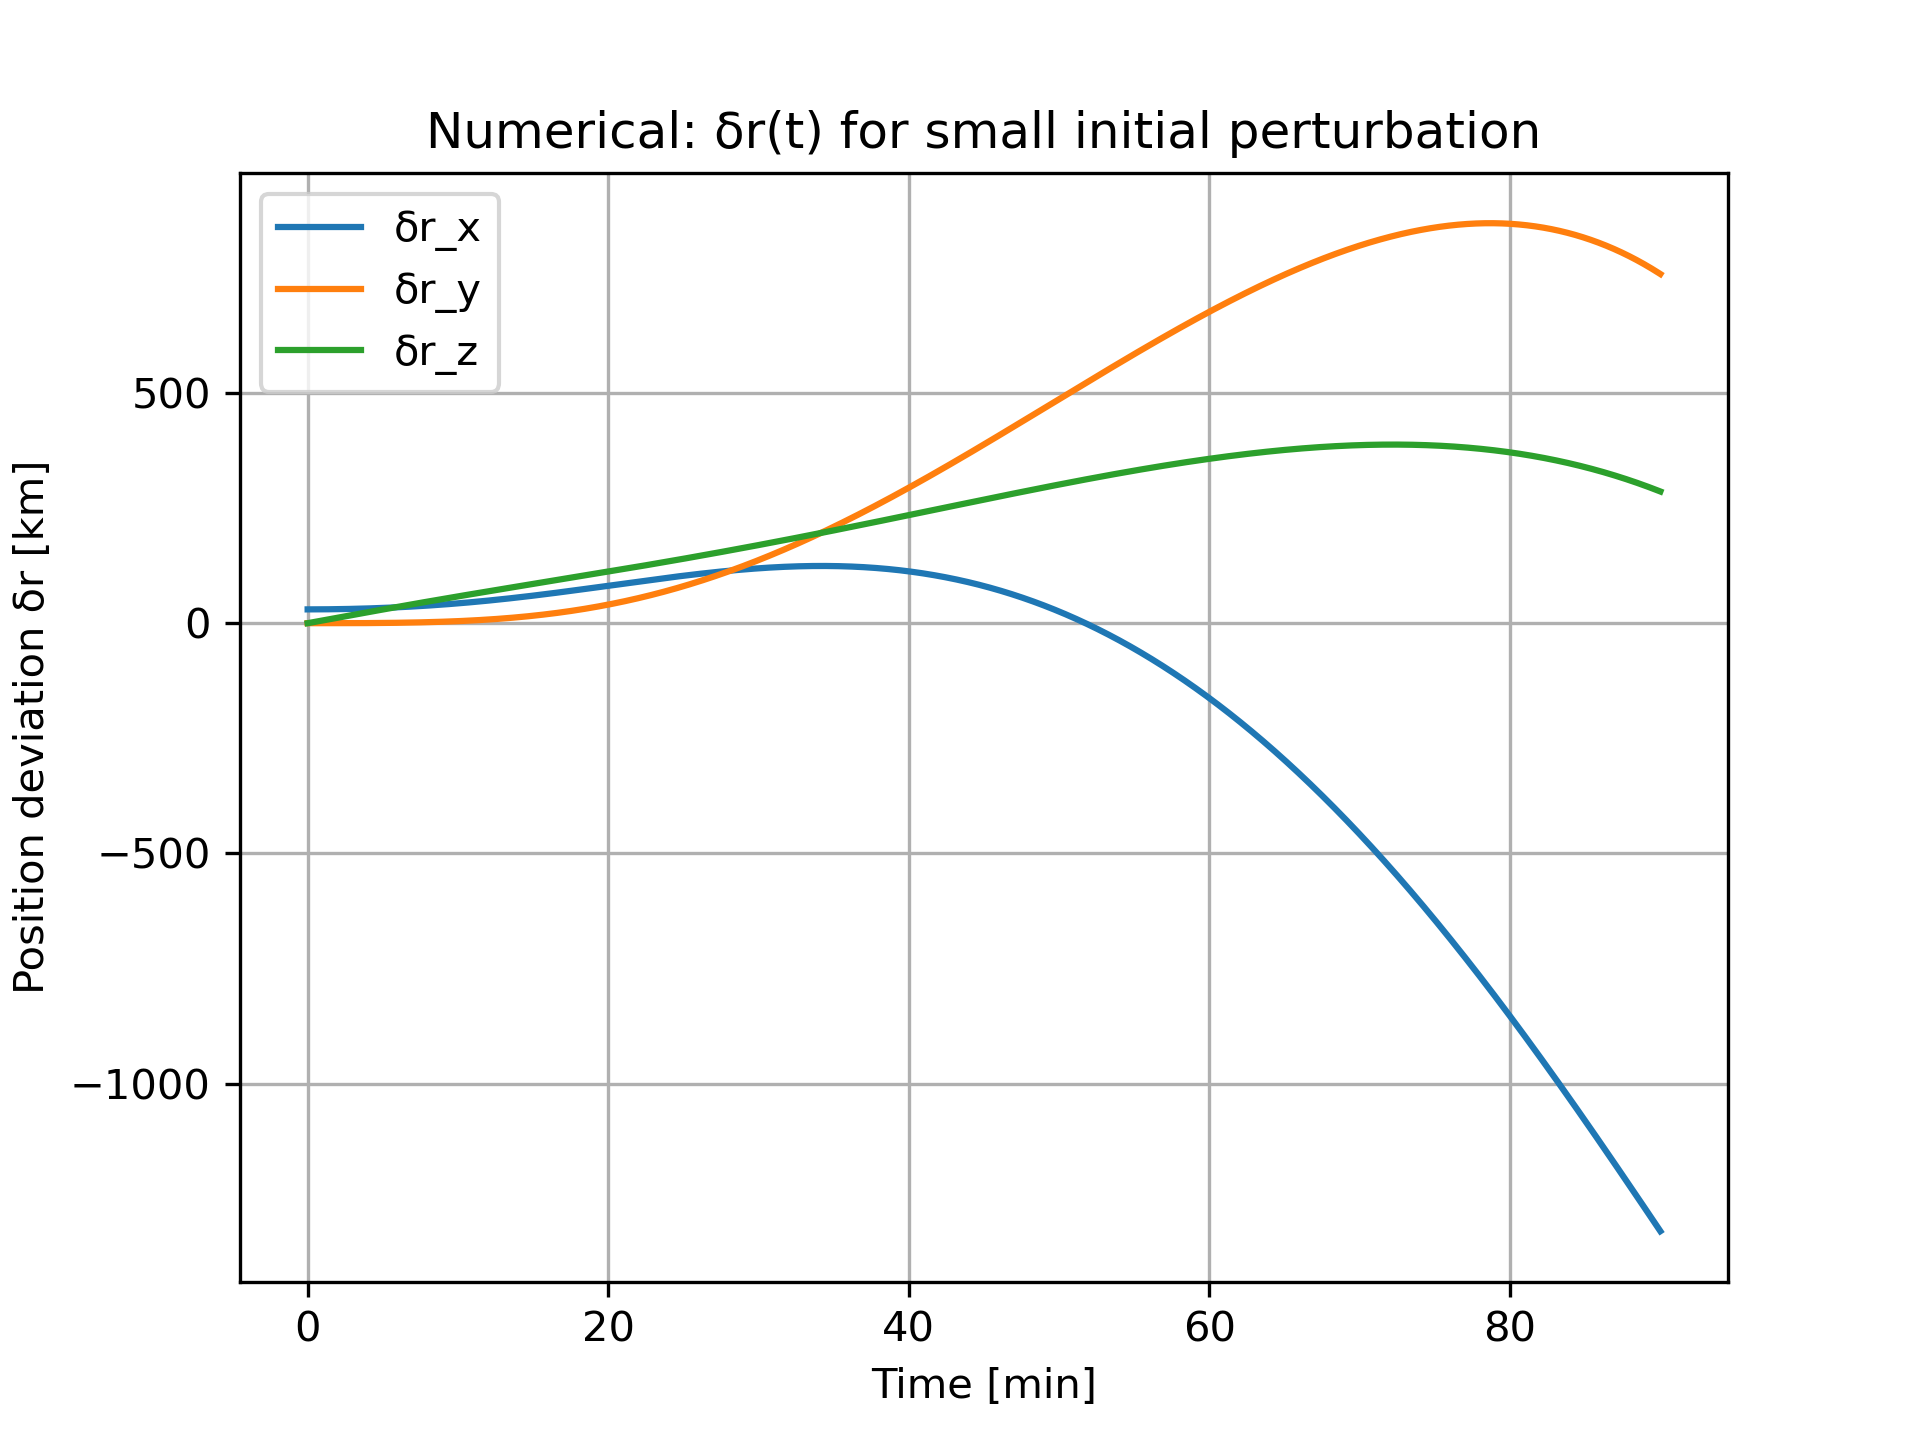
\includegraphics[width=0.45\textwidth]{./outputs/figures/s03d.png}
		\end{center}
		\caption{Numerical Integration \( \mathrm{d}\bm{X} \)}
	\end{figure}

	\hwkPart{} \label{hwk:s03e}

	\begin{figure}[H] \label{fig:s03e}
		\begin{center}
			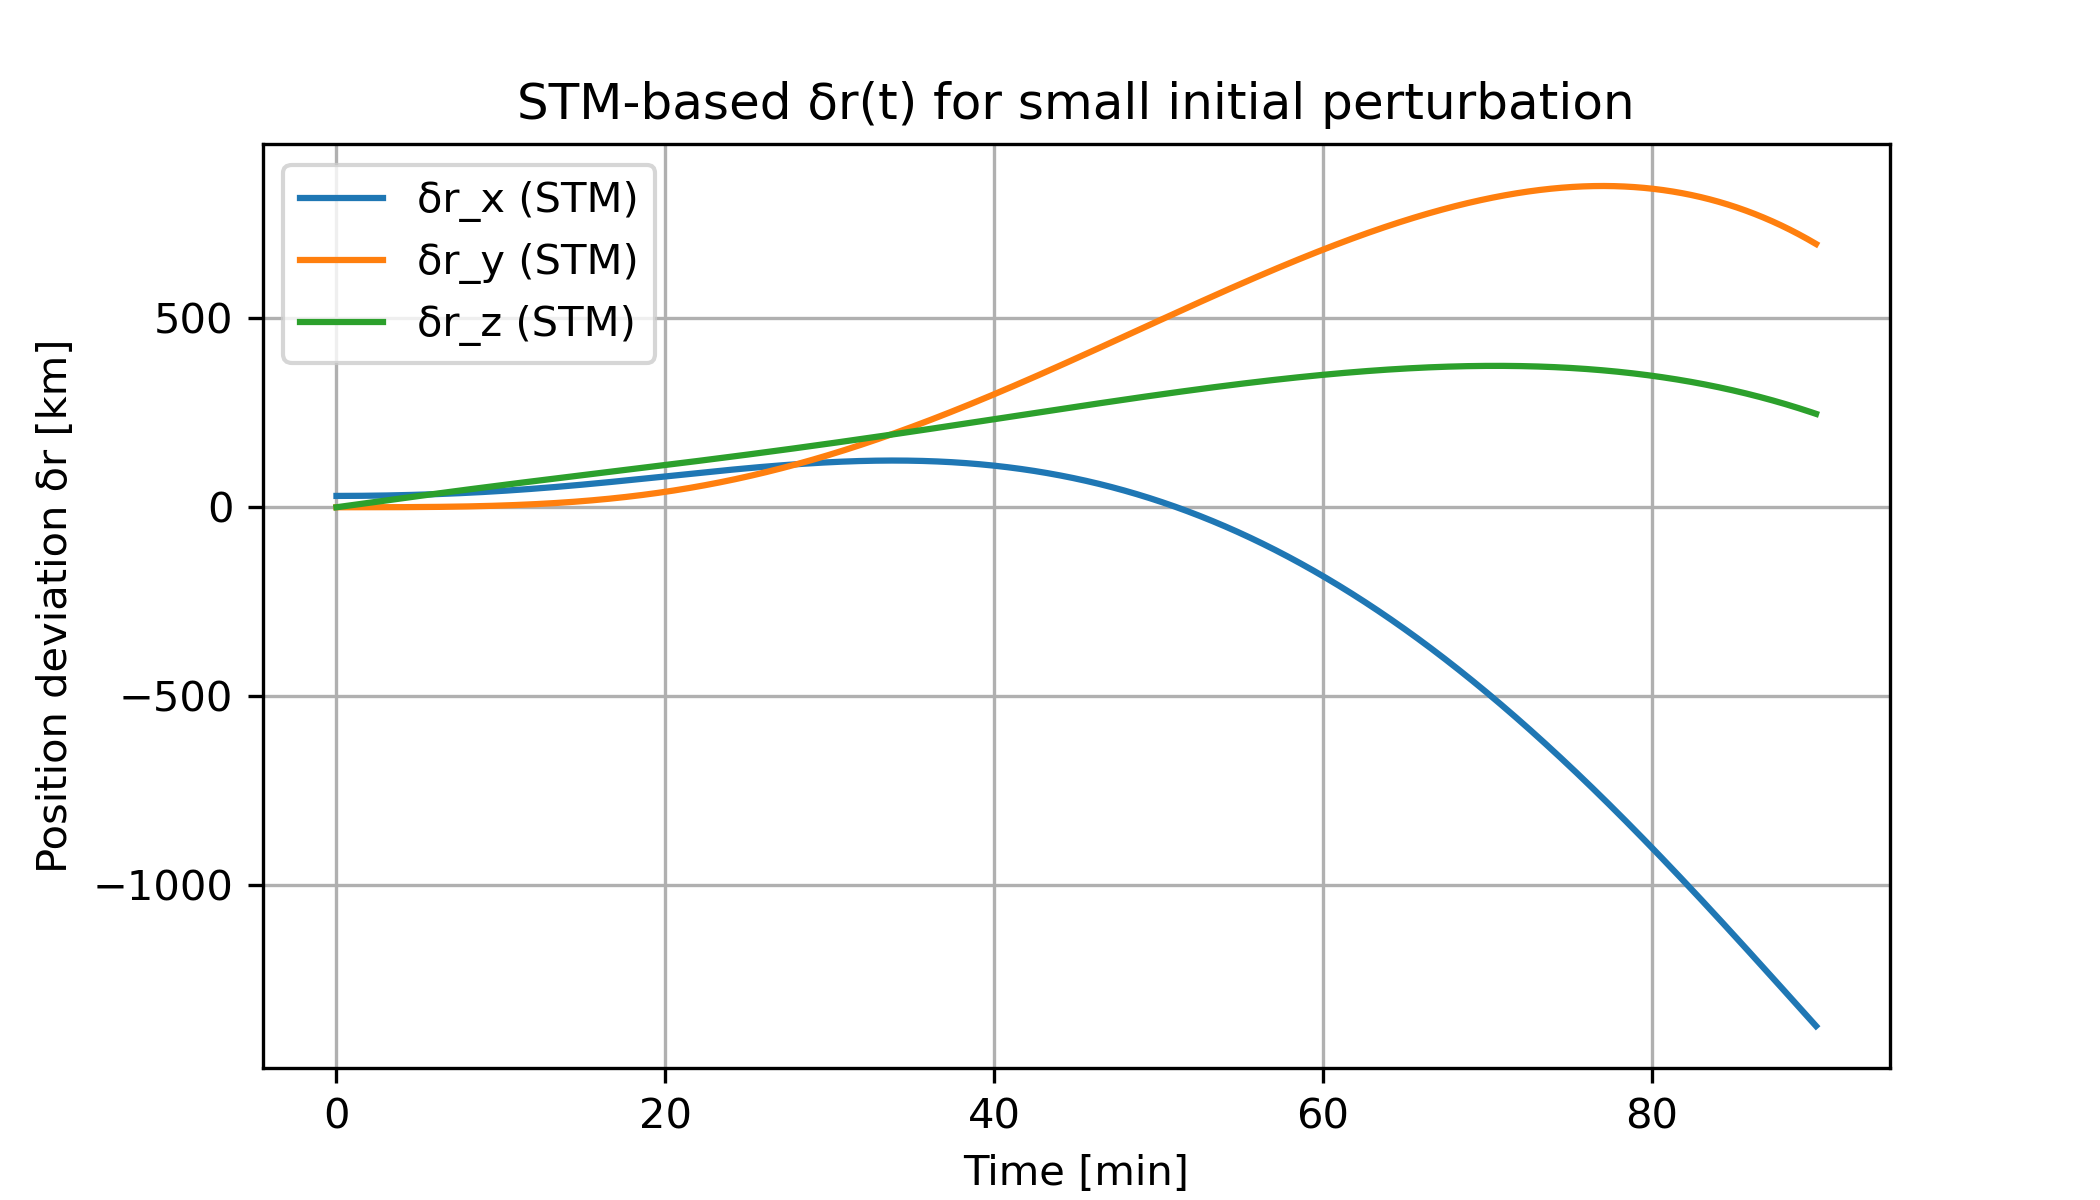
\includegraphics[width=0.45\textwidth]{./outputs/figures/s03e.png}
		\end{center}
		\caption{Analytic Integration \( \mathrm{d}\bm{X} \)}
	\end{figure}

	\hwkPart{} \label{hwk:s03f}

	\begin{figure}[H] \label{fig:s03f}
		\begin{center}
			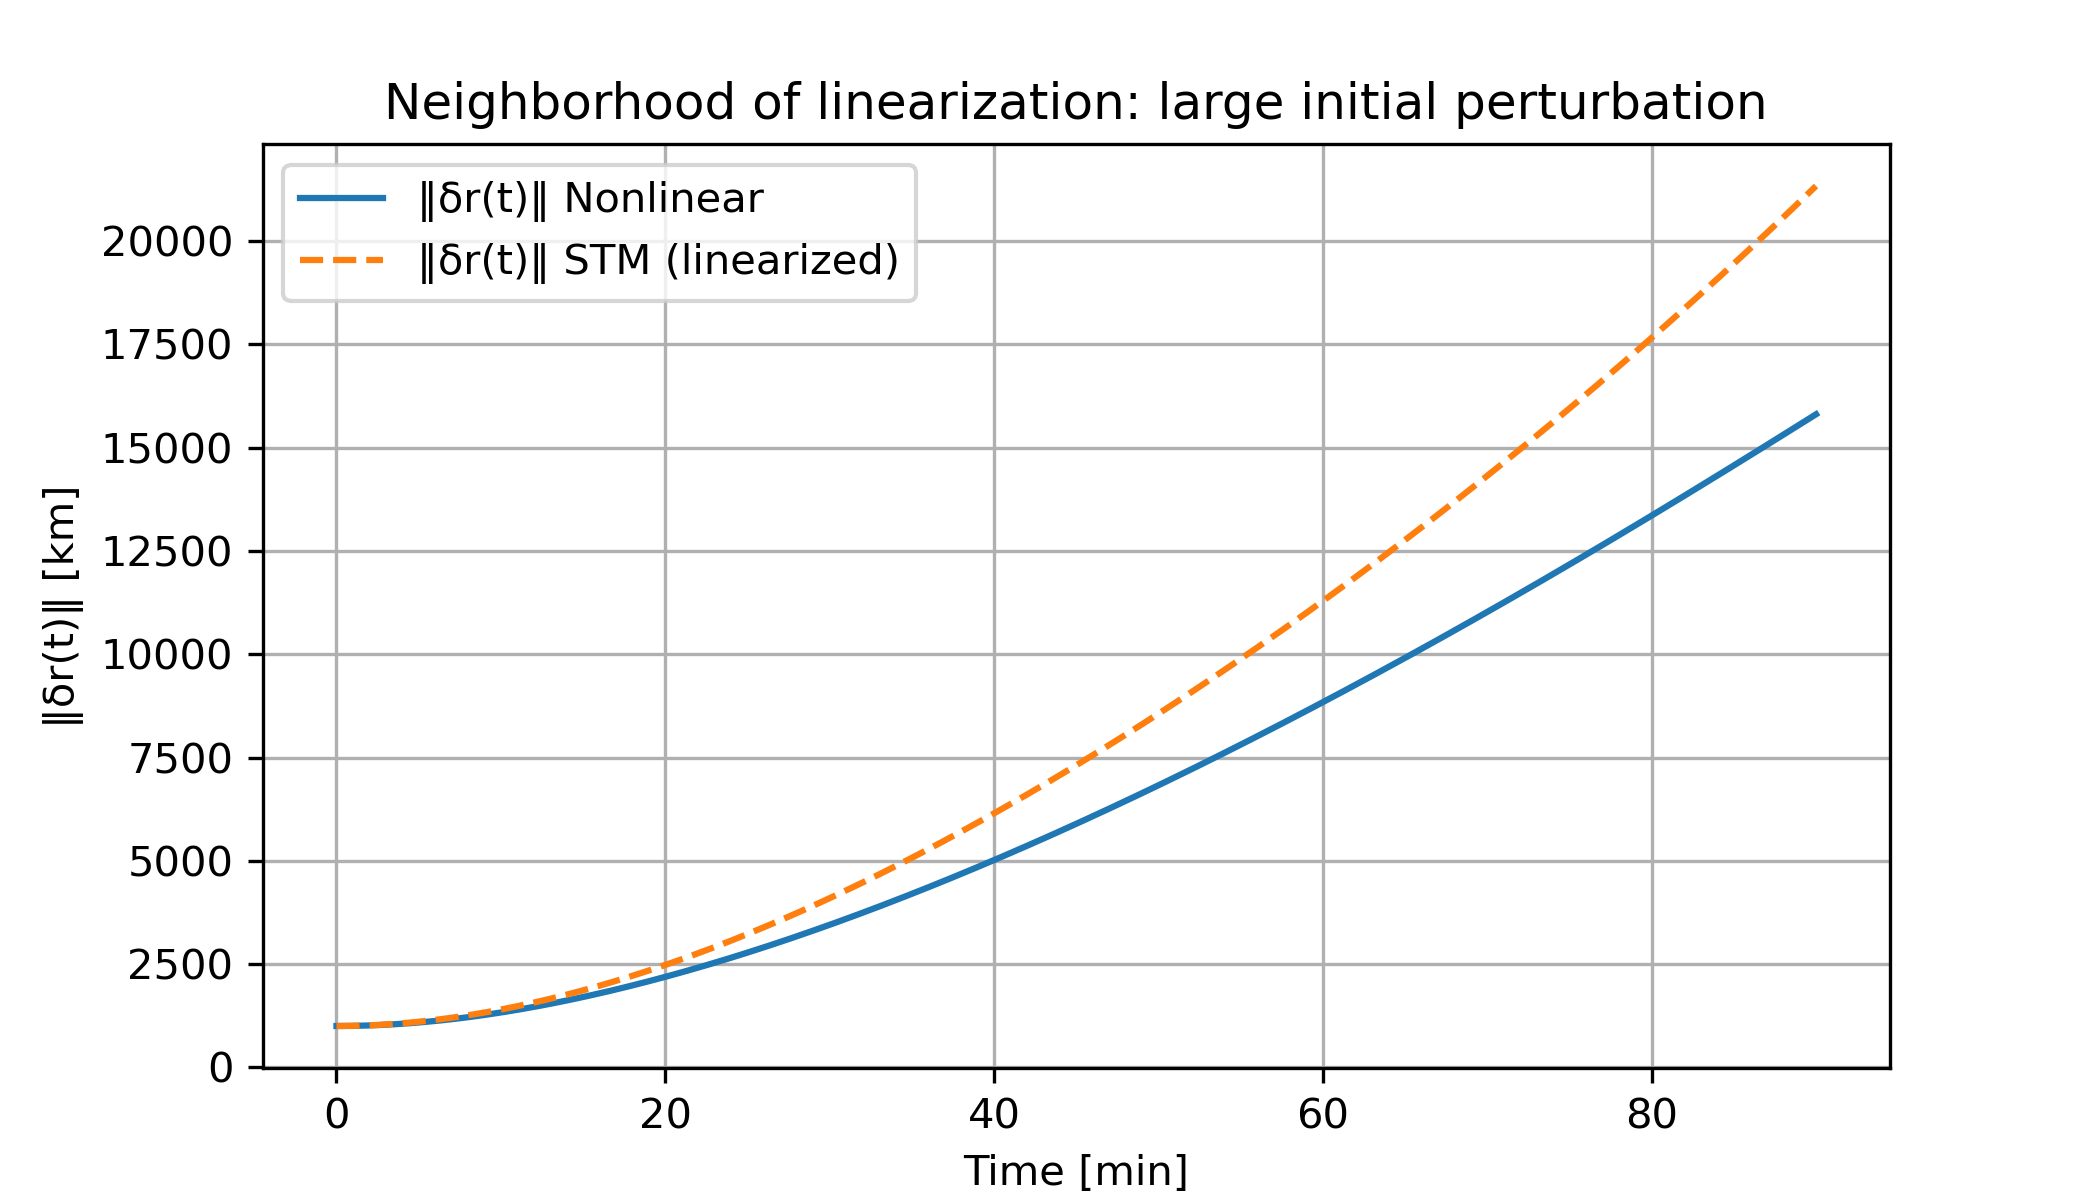
\includegraphics[width=0.45\textwidth]{./outputs/figures/s03f.png}
		\end{center}
		\caption{Critical \( \mathrm{d}\bm{X}_{\text{neighborhood}} \)}
	\end{figure}

	\hwkPart{} \label{hwk:s03g}

	\inputminted{python}{./outputs/text/s03g.txt}

	\hwkPart{} \label{hwk:s03h}

	\inputminted{python}{./outputs/text/s03h.txt}

	\hwkPart{} \label{hwk:s03i}

	\inputminted{python}{./outputs/text/s03i.txt}

	\hwkCode{} \label{code:s03}

	See the \href{https://www.github.com/vaisriv/enae441-hw03/blob/main/src/hw03.py#L347}{Python code} for this assignment.

\end{hwkProblem}

\end{document}
